\chapter{Median Finding in Linear Time}

\begin{algoprob}
	\problemtitle{\textsc{Median-Find}($S$)}
	\probleminput{Set $S$ of $n$ distinct integers}
	\problemquestion{Find the $\lt\lfloor\frac{n}{2}\rt\rfloor^{th}$ smallest integer in $S$}
\end{algoprob}

\section{Naive Algorithm}
The naive algorithm for this will be to sort the array in $O(n\log n)$ time then return the  $\lt\lfloor\frac{n}{2}\rt\rfloor^{th}$ element. This will take $O(n\log n)$ time. But in the next section we will show a linear time algorithm.

\section{Linear Time Algorithm}
In this section we will show an algorithm to find the median of a given set of distinct integers in $O(n)$ time complexity. We will follow \cite[Section 9.3]{CormenThomasLeisersonCharlesRivestRonaldSteinClifford_BOOK}. Consider the following two problems:

\begin{algoprob}
	\problemtitle{\textsc{Rank-Find} ($S,k$)}
	\probleminput{Set $S$ of $n$ distinct integers and an integer $k\leq n$}
	\problemquestion{Find the $k^{th}$ smallest integer in $S$}
\end{algoprob}
\begin{algoprob}
	\problemtitle{\textsc{Approximate-Split}($S$)}
	\probleminput{Set $S$ of $n$ distinct integers}
	\problemquestion{Given $S$, return an integer $z\in S$ such that $z$ where $rank(z)\in \lt[\frac{n}{4},\frac{3n}{4}\rt]$}
\end{algoprob}

%Certainly \prb{Rank-Find}$(S,k)$ is harder than $\prb{Approximate-Split}$. 
\subsection{Solve \prb{Rank-Find} using \prb{Approximate-Split}}
%Here suppose we can solve $\prb{Approximate-Split}$ easily. Now we want to solve $\prb{Rank-Find}$ using $\prb{Approximate-Split}$.
\begin{algorithm}
	\DontPrintSemicolon
	\KwIn{Set $S$ of $n$ distinct integer and $k\in[n]$}
	\KwOut{$k^{th}$ smallest integer in $S$}
	\Begin{
%$n\longleftarrow |S|$\;
\If{$|S|\leq 100$}{Sort $S$, \Return{$k^{th}$ smallest element in $S$}}	
$z\longleftarrow \prb{Approximate-Split}(S)$\hspace{1cm}
($z$ is the $r^{th}$ smallest element for some $r\in \lt[\frac{n}{4},\frac{3n}{4}\rt]$)\;
$S_L\longleftarrow \{x\in S\mid x\leq z\}$, $S_R\longleftarrow \{x\in S\mid x>z\}$\;
\If{$k\leq |S_L|$}{\Return{\prb{Rank-Find}$(S_L,k)$}}
\Return{\prb{Rank-Find}$(S_R,k-|S_L|)$}
}
\caption{\prb{Rank-Find}(S,k)}
\end{algorithm}
\parinn

Certainly if we can solve $\prb{Rank-Find}(S,k)$ for all $k\in[n]$ we can also solve $\prb{Median-Find}$. We will try to use both the problems and recurse to solve \prb{Rank-Find} in linear time. 

In the above algorithm $rank(z)\in \lt[\frac{n}{4},\frac{3n}{4}\rt]$. So $\frac{n}4\leq |S_L|,|S_R|\leq \frac{3n}4$. For now suppose $\prb{Rank-Find}(S,k)$ takes $T_{RF}(n)$ time and $\prb{Approximate-Split}(S)$ takes $T_{AS}(n)$ time. Then the time taken by the algorithm is  $$T_{RF}(n)\leq O(n)+T_{AS}(n)+T_{RF}\lt(\frac{3n}4\rt)$$
\subsection{Solve \prb{Approximate-Split} using \prb{Rank-Find}}
We first divide $S$ into groups of $5$ elements. So take $t=\lt\lceil\frac{n}5\rt\rceil$. Now we sort each group. Since each group have constant size this can be done in $O(n)$ time. So now consider the scenario:
\begin{figure}[h]
	\centering
	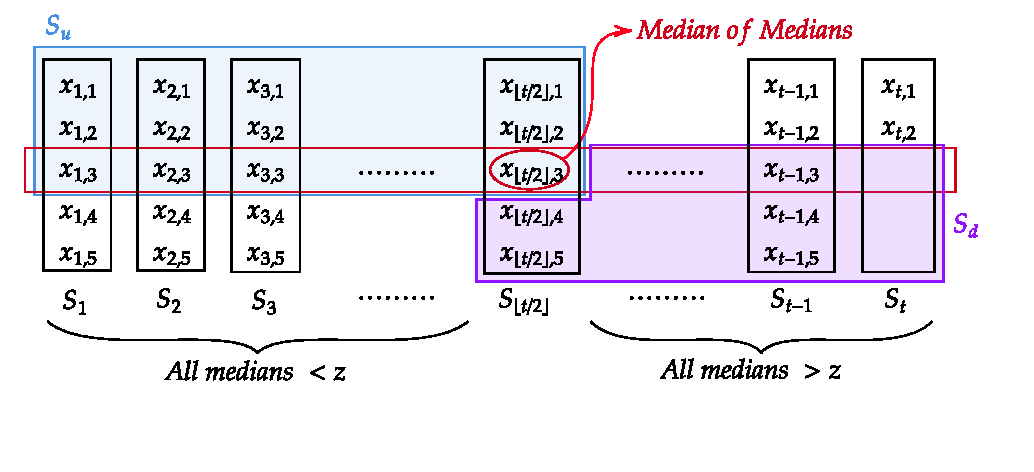
\includegraphics{images/approx-split-using-rankfind}
\end{figure}

After sorting each of the groups we takes the medians of each group. Let $x_{i,3}$ be the median of the medians. We claim that $rank(x_{i,3})\in  \lt[\frac{n}{4},\frac{3n}{4}\rt]$. 

\begin{algorithm}
	\DontPrintSemicolon
	\KwIn{Set $S$ of $n$ distinct integers}
	\KwOut{An integer $z\in S$ such that $z$ where $rank(z)\in \lt[\frac{n}{4},\frac{3n}{4}\rt]$}
	\Begin{
		\If{$|S|\leq 100$}{Sort, \Return{Exact median}}
		$t\longleftarrow\lt\lceil\frac{n}{5}\rt\rceil$\;
		$S_i\longleftarrow i^{th}$ block of 5 elements in $S$ for $i\in [t-1]$\; $S_t\longleftarrow$ Whatever is left in $S$\;
		\For{$i\in [t]$}{Sort $S_i$, Let $h_i$ be the median of $S_i$}
		$T\longleftarrow \{h_i\mid i\in[t]\}$\;
		\Return{$\prb{Rank-Find}\lt(T,\lt\lfloor \frac{t}{2}\rt\rfloor\rt)$}\;
	}
\caption{\prb{Approximate-Split}$(S)$}
\end{algorithm}

So in the picture among elements in upper left the highest element is $x_{i,3}$ and among the elements in lower right the lowest element is $x_{i,3}$. We will show that the number of elements smaller than $x_{i,3}$ is between $\frac{n}{4} $ and $\frac{3n}{4}$. Lets call the set of elements in upper left box is $S_u$ and the set of elements in lower right box is $S_d$.

\begin{lemma}{}{}
	$|S_u|,|S_d|\geq\frac{n}{4}$
\end{lemma}
\begin{proof}
	$|S_u|\geq 3\times \lt\lfloor\frac{t}{2}\rt\rfloor$. For $n\geq 100$, $3\lt\lfloor\frac{t}{2}\rt\rfloor> \frac{n}{4}$. Hence $|S_u|\geq \frac{n}{4}$. Now similarly $|S_d|\geq 3\lt\lfloor\frac{t}{2}-1\rt\rfloor\geq \frac{n}{4}$.
\end{proof}
\begin{lemma}{}{}
	Number of elements in $S$ smaller than $x_{i,3}$ lies between $\frac{n}4$ and $\frac{3n}{4}$.
\end{lemma}
\begin{proof}
	Now number of elements in $S$ smaller than $x_{i,3}\geq |S_u|\geq \frac{n}4$. The number of elements greater than $x_{i,3}\geq |S_d|\geq \frac{n}{4}$. So number of elements in $S$ smaller than $x_{i,3}\leq n-$ number of elements greater than $x_{i,3}\leq n-\frac{n}4=\frac{3n}{4}$.
\end{proof}
Hence the \prb{Approximate-Split}$(S)$ takes time $$T_{AS}(n)=O(n)+T_{RF}\lt(\frac{n}{5}\rt)$$
\subsection{Time Complexity}
Replacing $T_{AS}(n)$ in the time complexity equation of $T_{RF}(n)$ we get the equation:$$T_{RF}(n)\leq O(n)+T_{RF}\lt(\frac{n}5\rt)+T_{RF}\lt(\frac{3n}{4}\rt)$$Let $T_{RF}(n)\leq kn++T_{RF}\lt(\frac{n}5\rt)+T_{RF}\lt(\frac{3n}{4}\rt)$. We claim that $T_{RF}(n)\leq cn$ for some $c\in \bbN$ for all $n\geq n_0$ where $n_0\in \bbN$. By induction we have $$T_{RF}(n)\leq kn+\frac{cn}{5}+\frac{3cn}{4}=\lt(k+\frac{19c}{20}\rt)n$$To have  $k+\frac{19c}{20}\leq c$ we have to have $k+\frac{19c}{20}\leq c\iff c\geq 20k$. So take $c\geq 20k$ and our claim follows. Hence $T_{RF}(n)=O(n)$. Since we can find any $k^{th}$ smallest number in a given set of distinct integers in linear time we can also find the median in linear time.